Στο κεφάλαιο αυτό αρχικά αναφέρονται κάποιες εφαρμογές που χρησιμοποιούνται παγκοσμίως σήμερα, για την διαχείριση έργων.Στην συνέχεια, περιγράφεται σε γενικές γραμμές η εφαρμογή \e{iPM}, η αρχιτεκτονική της και ύστερα οι λειτουργίες της ως προς των κώδικα.

\section{Έρευνα αγοράς}

\subsection{\e{Asana}}
\quadΤο \e{Asana} είναι ίσως η πιο γνωστή εφαρμογή που έχει σχεδιαστεί για να βοηθήσει τις ομάδες να παρακολουθούν τα έργα τους.\\
\pSpaceΚάθε ομάδα μπορεί να δημιουργήσει ένα χώρο εργασίας. Οι χώροι εργασίας περιέχουν έργα και τα έργα περιέχουν εργασίες. Σε κάθε εργασία, οι χρήστες μπορούν να προσθέτουν σημειώσεις, σχόλια, συνημμένα και ετικέτες. Οι χρήστες μπορούν να ακολουθήσουν τα έργα και τις εργασίες και, όταν αλλάξει η κατάσταση ενός έργου ή μιας εργασίας, οι ακόλουθοι λαμβάνουν ενημερώσεις σχετικά με τις αλλαγές στα εισερχόμενά τους. \e{\parencite{asana_wiki}} Αυτό βοηθάει την παρακολούθηση των εργασιών από την αρχή μέχρι το τέλος, την ανάθεση υποεργασιών σε μέλη της ομάδας και τον καθορισμό προθεσμιών για να διασφαλιστεί ότι τα έργα θα γίνουν εγκαίρως. Έτσι ομάδες εργάζονται πιο παραγωγικά και αποτελεσματικά.\e{\parencite{asana_task}}\\
\pSpaceΈνα άλλο πολύ σημαντικό χαρακτηριστικό αυτής της εφαρμογής είναι το ότι προσφέρει την δυνατότητα να χρησημοποιηθεί το \e{API} τους απο τρίτους.Επομένως, εφαρμογές όπως \e{Dropbox, Evernote, GoogleDrive, Instagantt, Jira} και άλλα, μπορούν να συνδεθούν με τον λογαριασμό \e{Asana}, ετσι ώστε να μεγαλώσει την παραγωγικότητα του χρήστη.

\subsection{\e{Trello}}
\pSpaceΆλλη μια διαδικτυακή εφαρμογή που αξίζει να σημειωθεί είναι το \e{Trello}, τωρα υπό το όνομα \e{Attlassian}.Το απλό \e{design} και η δυνατότητα \e{Agile} κέρδισε πελάτες πολύ εύκολα.\\
\pSpaceΕπίσης η ικανότητα να συνδέσει κανείς το \e{dashboard} με υπηρεσίες όπως \e{Slack, GitHub} φέρνει ένα σημαντικό πλεονέκτημα σε σχέση με άλλες εφαρμογές. 

\section{\e{iPM} - Γενική Περιγραφή}
\pSpace'Οπως προαναφέρθηκε, ο σκοπός της πτυχιακής είναι η ανάπτυξη μιας διαδικτυακής εφαρμογής για την διαχείριση έργων, το οποίο ονομάστηκε \e{iPM}.\\
\pSpaceΟ χρήστης δημιουργεί έναν λογαριασμό για να έχει πρόσβαση στην εφαρμογή, όπου μπορεί να δημιουργήσει καινούργια πρότζεκτ η να διαχειρίσει ήδη υπάρχοντα αν είναι μέλος η διαχειριστής αυτόν.Για να συμβάλλει σε κάποιο άλλο έργο, θα πρέπει να τον καλέσει κάποιο μέλος, και αφού δεχτεί θα μπορέσει να δεί λεπτομέριες, να του ανατεθούν εργασίες, η να πάρει μέρος στις συζητήσεις που αφορούν το συγκεκριμένο έργο.\\
\pSpaceΟ χρήστης μπορεί να παρακολουθεί την πρόοδο του έργου μέσα απο τα διαγραμμάτα στον χώρο εργασίας έργου, η απο τα διαγράμματα Γκαντ.Επίσης κάθε μέλος ενημερώνεται άμεσα για κάθε ένεργεια που τον αφορά προσωπικά.

\subsection*{\e{Use Cases}}
\pSpaceΣτο παρακάτω \e{UML} διάγραμμα φαίνονται τα βασικά \e{Use Cases} της εφαρμογής.
\begin{figure}[ht]
\centering
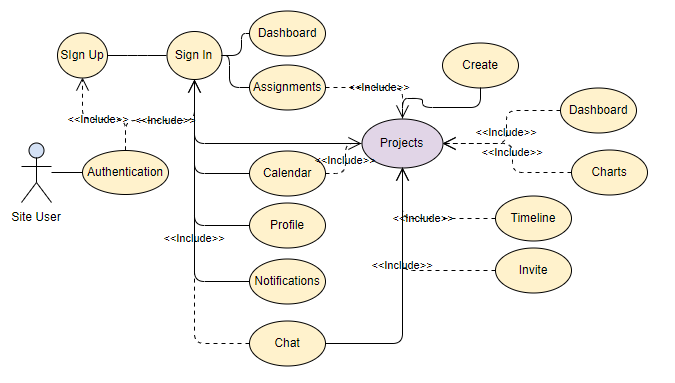
\includegraphics[scale=1]{images/usecase.jpg}
\caption{\e{UML Use Cases}}
\label{fig:use_cases}
\end{figure}
\pagebreak

\subsection*{Χάρτης Εφαρμογής - \e{Site map}}
\dirtree{%
.1 \e{Homepage}.
.1 \e{Auth}.
.2 \e{Sign Up}.
.3 \e{Sign In}.
.1 \e{App}.
.2 \e{Dashboard}.
.2 \e{My Projects}.
.3 \e{Project}.
.4 \e{Dashboard}.
.4 \e{Assignments}.
.5 \e{Classic}.
.5 \e{Agile}.
.4 \e{Gantt}.
.4 \e{Team}.
.4 \e{Timeline}.
.4 \e{Chat}.
.4 \e{Settings}.
.2 \e{My Tasks}.
.2 \e{My Issues}.
.2 \e{Calendar}.
.2 \e{Chat}.
.2 \e{Profile}.
.2 \e{Invites}.
}

\subsection*{Υποθέσεις και εξαρτήσεις}
\pSpaceΔεδομένου ότι είναι μια διαδικτυακή εφαρμογή, το τελικό προιόν θα είναι προσβάσιμο μέσω ίντερνετ απο περιηγητή ιστού (\e{Web Browser}) τελευταίας έκδοσης.Δέν υποστηρίζεται δυνατότητα \e{offline}.

\section{\e{Specific Requirements}}
\subsection*{\e{User Stories}}
\pSpaceΌπως προκύπτει και απο σχ. \ref{fig:use_cases} τα \e{User Stories} πηγαίνουν ως εξής:
\begin{itemize}
	\item Ο χρήστης μπορεί να δημιουργήσει έναν λογαριασμό παρέχοντας μια ηλεκτρονική διεύθυνση (\e{email}) και κωδικό.
	\item Η σύνδεση στην εφαρμογή επιτυγχάνεται με τα δεδομένα που προμηθεύτηκαν στο στάδιο εγγραφής.
	\item Στον χώρο εργασίας χρήστη φαίνονται τα \e{assignments} που χρειάζονται την προσοχή όπως και συντομεύσεις για τα έργα στα οποία είναι μέλος.
	\item Επίσης ο χρήστης μπορεί να δεί τις εργασίες που του αναθέτηκαν ανά τύπο (\e{Task/Issue}) και να χρησιμοποιήσει την συντόμευσή της.
	\item Ακόμη, έχει την δυνατότητα να αλλάξει τις πληροφορίες μέσα απο το \e{Profile}
	\item Στο \e{Calendar} φαίνονται όλα τα γεγονότα, είτε προσωπικά η κάποιου έργου.
	\item Οι ειδοποιήσεις έχουν πρόσβαση από παντού, και καλύπτουν τα γεγονότα που χρειάζονται προσοχή.
	\item Επιπλεόν στο \e{Chat} υπάρχουν όλες οι συζητήσεις έργων, και ο χρήστης μπορεί να συμβάλλει σε αυτά σε πραγματικό χρόνο.
	\item Ο χρήστης φυσικά μπορεί να δημιουργήσει και να διαχειρίσει έργα.
	\item Έχει την δυνατότητα να καλέσει χρήστες που έχουν λογαριασμό στην εφαρμογή, σε κάποιο έργο.
	\item Επιπροσθέτως, μπορεί να αναθέτει εργασίες στά μέλοι έργου.
	\item Για την καλύτερη και ομαλότερη εμπειρία, ο χρήστης μπορεί να φιλτράρει τις εργασίες με βάση όνομα, μέλοι, κατάσταση η/και τύπο.
	\item Ο διαχειριστής μπορεί να δεί και να αλλάξει τις πληροφορίες η ρυθμίσεις έργου.
	\item Ο χρήστης μπορεί να παρακολυθεί την πρόοδο με οπτικό τροπο, απο τα διαγράμματα.Επίσης μπορεί να αποθηκεύσει στην συσκεύη κάποιο διάγραμμα για άλλη χρήση.
\end{itemize}

\subsection*{\e{System Requirements}}
\pSpaceΗ εφαρμογή ανήκει στην γενιά \e{Web 2.0} εφόσον είναι \e{Centralized} τύπου.Οπότε, για τους σκοπούς αυτής της πτυχιακής εργασίας, το δωρεάν \e{domain} της \e{Heroku} και την επίσης δωρεάν έκδοση της \e{mLab} καλύπτουν πλήρως τις ανάγκες της εν λόγω εφαρμογής.
\pagebreak

\section{Αρχιτεκτονική}

\subsection*{Δομή του έργου}
\pSpaceΤο πρότζεκτ έχει την ακόλουθη δομή:\\
\dirtree{%
.1 \e{iPM}.
.2 \e{src}.
.3 \e{client}.
.3 \e{config}.
.3 \e{e2e}.
.3 \e{server}.
.3 \e{main.ts}.
.2 \e{.angular-cli.json}.
.2 \e{.editorcofig}.
.2 \e{package.json}.
.2 \e{tsconfig.json}.
.2 \e{tslint.json}.
.2 \e{typings.json}.
.2 \e{webpack.config.js}.
.2 \e{.gitignore}.
}

\pSpaceΟ φάκελος \e{src} περιλαμβάνει όλη την εφαρμογή, \e{front-end} και \e{back-end}, ενώ τα υπόλοιπα αρχεία προμηθεύουν τις ρυθμίσεις και τα απαραίτητα για την εγκατάστση της εφαρμογής.\\
\pSpaceΣυγκεκριμένα:
\begin{itemize}
	\item Στο \e{.angular-cli.json} προσθέτονται οι εφαρμογές που θα τρέξουν, και για την κάθε μια ρυθμίζονται που θα αποθηκεύτει το έτοιμο πακέτο, ποιο έιναι τα \e{root} όσον αφορά την \e{main, index, polyfills, test} και καθολικά στύλ.Δηλαδή εδώ υπάρχουν οι αναφορές για οτι αφορά τις εφαρμογές \e{Angular}.
	\item \e{.editorconfig} κρατάει τις ρυθμίσεις για το \e{coding-style} που χρησιμοποιείται.Αυτό σημαίνει πώς αν αυτό το πρότζεκτ θα ανοιχτεί σε ενα διαφορετικό \e{IDE} από αυτό στο οποίο δημιουργήθηκε, ο κώδικας θα φανεί όπως είναι αναμενόμενο, με τα σωστά κενά κλπ.
	\item Το αρχείο \e{package.json} αποθηκεύει τα \e{script} που κατασκεύαζουν η τρέχουν την εφαρμογή, αλλά και τις εξαρτήσεις.
	\item Στο \e{tsconfig.json} βρίσκονται οι απαραίτητες ρυθμίσεις για το \e{TypeScript}, εφόσον η εν λόγω εφαρμογή γράφτηκε χρησιμοποιώντας αυτό το \e{super-script} της \e{JavaScript}.
	\item Δεδομένου ότι ασχολήθηκαν δύο άτομα στην ανάπτυηξη της εφαρμογής, για μια ομαλότερη εμπειρία, χρησιμοποίηθηκε το \e{TypeScript Lint}, έτσι ώστε να κυριαρχεί ένα \e{Coding Style}. 
	\item Οι ρυθμίσεις του \e{module builder, Webpack}, βρίσκονται στο αντίστοιχο αρχείο \e{.js}.
	\item Τελευταίο, το αρχείο \e{.gitignore} χρειάστηκε τόσο για το \e{GitHub} αλλά και για το \e{Heroku}, όπου ανεβάσαμε την εφαρμογή.Με αυτόν τον τρόπο ανεβαίνουν μόνο τα απαραίτητα αρχεία.
\end{itemize}
\pSpaceΣτρέφοντας την προσοχή πίσω στον φάκελο \e{src}, παρατηρούνται τα εξής:
\dirtree{%
.1 \e{src}.
.2 \e{client}.
.2 \e{config}.
.2 \e{e2e}.
.2 \e{server}.
.2 \e{main.ts}.
}
\pSpaceΟ φάκελος \e{client} περιλαμβάνει το \e{front-end}, στο \e{e2e} βρίσκονται τα \e{test} ενώ τα υπόλοιπα αποτελούν τον \e{server}.

\pSpaceΤο αρχείο \e{main.ts} είναι υπεύθυνο για να ξεκινήσει ο \e{server}, η βάση δεδομένων και το \e{Socket.io}, όπως και την διαχείρηση των διαδρομών.Εφόσον η εφαρμογή είναι \e{One-Page Application} οποιαδήποτε διαδρομή εκτός του \e{/api...} θα απασχολείται απο το \e{Angular}.\\
\pSpaceΠαρακάτω φαίνονται τα περιεχόμενα του φακέλου \e{server}: 
\dirtree{%
.1 \e{server}.
.2 \e{database}.
.3 \e{dbClient.ts}.
.3 \e{utils.ts}.
.2 \e{routes}.
.3 \e{assignments}.
.3 \e{auth.ts}.
.3 \e{calendar.ts}.
.3 \e{chat.ts}.
.3 \e{invite.ts}.
.3 \e{notifications.ts}.
.3 \e{project.ts}.
.3 \e{settings.ts}.
.3 \e{timeline.ts}.
.3 \e{user.ts}.
.2 \e{controller.ts}.
.2 \e{socket.ts}.
.2 \e{utils.ts}.
}

\pSpaceΣυνεχίζοντας στο κομμάτι του \e{client}, παρατηρείται η επόμενη δομή:
\dirtree{%
.1 \e{client}.
.2 \e{app}.
.2 \e{assets}.
.2 \e{index.html}.
.2 \e{karma.conf.js}.
.2 \e{main.server.ts}.
.2 \e{main.ts}.
.2 \e{polyfills.ts}.
.2 \e{test.ts}.
.2 \e{tsconfig.app.json}.
.2 \e{tsconfig.server.json}.
.2 \e{ts.config.spec.json}.
.2 \e{typings.d.ts}.
}
\pSpaceΣτον φάκελο \e{app} βρίσκονται όλα τα \e{component}, ενώ στο \e{assets} περιλαμβάνονται τα καθολικά \e{scss} και εικόνες οι οποίες χρησιμοποιήθηκαν στην εφαρμογή.\\
\pSpaceΤο \e{index.html} είναι η σελίδα στην οποία θα προσθετεί το δυναμικό περιεχόμενο.Περιέχει τα απαραίτητα \e{metadata}, διευθύνσεις για εικονίδια, διαγράμματα και το \e{tag "app-root"} που αφορά το περιεχόμενο της εφαρμογής.Στα υπόλοιπα αρχεία βρίσκονται οι ρυθμίσεις του \e{Angular}, \e{test} και \e{Typescript}.
\selectlanguage{greek}
\section{Αναλυτική περιγραφή της εφαρμογής}
\pSpaceΣε αυτό το υποκεφάλαιο, περιγράφονται αναλυτικά τα σημαντικά κομμάτια της εφαρμογής.Ξεκινώντας με τον \e{server} και το\e{api}, στην συνέχεια θα αναφέρονται τα \e{component} του \e{front-end}, η δομή και η λογική τους, και στο τέλος η βάση δεδομένων.

\subsection{\e{Server}}
\pSpaceΟ \e{server} είναι γραμμένος σε \e{TypeScript} όπως και το υπόλοιπο της εφαρμογής και τρέχει πάνω σε πρωτόκολλο \e{HTTP} και περιβάλλον \e{NodeJS}.Επίσης προσθέτηκε και ένα \e{server Socket.io} το οποίο τρέχει παράλληλα με τον αρχικό, στο ίδιο \e{domain} και θύρα.\\
\pSpaceΤο \e{ExpressJS framework} βοηθάει στην καλύτερη οργάνωση του διακομιστή, αλλά ταυτόχρονα κάνει όλη την εμπειρία να κυλάει πιο ομαλά.Με την βοήθειά του, οι ρυθμίσεις για τον τύπο δεδομένων που στέλνονται και δέχονται, διαδρομές και μεθόδους επαλήθευσης πριν την πρόσβαση σε ενα συγκεκριμένο \e{endpoint}, επιτευχθονται με λιγότερο κώδικα.\\
\pSpaceΓια την καλύτερη οργάνωση, δημιουργήθηκε μια κλάση \e{IOServer} η οποία εξυπηρετεί μόνο το \e{Socket.io}.Αυτή η κλάση περιλαμβάνει ιδιωτικές μεταβλητές τα οποία αποθηκεύουν τα \e{id} των τρέχων \e{socket}/χρηστών, δωματιών (ενα δωμάτιο ανά έργο) αλλά και μεθόδους για αποστολή δεδομένων σε συγκεκριμένα δωμάτια.Ο \e{constructor} της παίρνει ως παράμετρο το αρχικό \e{server}, για να σιγουρεύτει ότι ξεκινάει όντως παράλληλα με τον πρώτο και στην συνέχεια περιμένει/<<ακούει>> για συγκεκριμένα μηνύματα που ανταλάσσονται στο \e{ioserver}.Για παράδειγμα, την στιγμή που ένας χρήστης συνδεέται στην εφαρμογή, λαμβάνεται ένα μήνυμα στο \e{io} διακομιστή μαζί με το \e{token} του χρήστη.Αν επαληθεύεται, ο χρήστης προσθίτεται στα δωμάτια που πρέπει να ανήκει, ετσι δίνωντας του την δυνατότητα να λαμβάνει σημαντικά γεγονότα σε πραγματικό χρόνο.Παρακάτω παρουσιάζονται δύο παραδείγματα που καλύπτουν την αποστολή και την λήψη δεδομένων πάνω σε \e{Socket.io}.\\
\pSpaceΓια την άποστολή δεδομένων υπάρχουν δύο τρόπους:
\begin{itemize}
	\item Στην περίπτωση που στέλνει στο <<τρέχων>> \e{socket}.
	\selectlanguage{english}
	\begin{lstlisting}[language=Java]
socket.emit('message', data); 
	\end{lstlisting}
	\selectlanguage{greek}
	\item Ενω όταν χρειάζεται να στείλει σε ένα δωμάτιο η σε συγκεκριμένους χρήστες.
	\selectlanguage{english}
	\begin{lstlisting}[language=Java]
this.io.to(this.clients[email]).emit('message', data);
	\end{lstlisting}
	\selectlanguage{greek}
\end{itemize}
\pSpaceΗ λήψη δεδομένων τόσο στο \e{server side} όσο και στο \e{client-side} επιχειρείται παρομοίως:
\selectlanguage{english}
	\begin{lstlisting}[language=Java]
	socket.on('message', data => {...});
	\end{lstlisting}
\selectlanguage{greek}

\pSpaceΑπόδειξη της χρησιμότητας του \e{Express} είναι η εισαγωγή διαδρομών του \e{api}.Σε μια γραμμή κώδικα, εισάγονται όλα όσα χρειάζονται οσον αφορά τα \e{back-end endpoints}.Ουσιαστικά, οποιαδήποτε διεύθυνση ξεκινάει με το \e{domain} ακολουθούμενο απο το \e{/api} θα ενεργοποιεί μια διαδρομή μονο.\\
\selectlanguage{english}
	\begin{lstlisting}[language=Java]
	app.use('/api', apiRouter);
	\end{lstlisting}
\selectlanguage{greek}
\pSpaceΣτην συνέχεια, η κλήση φτάνει στον \e{controller} ο οποίος έχει τον ρόλο να ανακατευθύνει τις κλήσεις στον τελικό προόρισμό τους, όχι πριν επαληθευτεί όμως το \e{token} η τα δεδομένα.Για παράδειγμα:\\
\selectlanguage{english}
	\begin{lstlisting}[language=Java]
router.use('/auth', checkBody, checkAccount, authRouter);
	\end{lstlisting}
\selectlanguage{greek}
\pSpaceΣτην παραπάνω γραμμή, αν η διεύθυνση είχε την μορφή <<\e{../api/auth}>>, ο διακομιστής καταλαβαίνει ότι αναφέρεται στα \e{endpoints} ταυτοποίησης.Πριν αποκτήσει πρόσβαση όμως, ελέγχει αν η κλήση \e{http} κατέχει δεδομένα, και στην συνέχεια αν αυτά τα δεδομένα έχουν την μορφή που αναμένεται, στην περίπτωση αυτή αν υπάρχει το αντικείμενο με κλειδί <<\e{account}>> και δεν είναι κενό ή λάθος.Οι μέθοδοι αυτοί λέγονται <<\e{Middleware Functions}>> και ο μέγιστος αριθμός του θεωρητικά μπορεί να είναι άπειρος.Με αυτόν τον τρόπο, αρνείται η περαιτέρω πρόσβαση στα \e{endpoints} και προβλήματα η τυχόν \e{bugs} που μπορεί να εμφανιστούν σε τέτοιες περιπτώσεις, δεν θα περάσουν.Επίσης, η εγγραφές/διάβασματα βάσης δεδομένων θα ελαχιστοποιούνται σημαντικά.\\
\pSpaceΠαρακάτω φαίνεται πως διαχειρίζεται μια κλήση μέθοδου \e{POST} στην διεύθυνση <<\e{/api/auth/signin}>>.Ο λόγος που το \e{callback function} είναι τύπου \e{async}, είναι επειδή η βάση δεδομένων υποστηρίζει \e{Promise}, και σε συνδυασμό των δύο ο κώδικας είναι πιο σίγουρο σε δύσκολες περιπτώσεις, εφόσον η \e{async} ακυρώνει τα περισσότερα μειωνεκτήματα τις \e{Promise}.\\
\pSpaceΤο αντικείμενο <<\e{res}>> στέλνει πίσω στο \e{client} την απάντηση που έχει, χρησιμοποιώντας κωδικούς κατάστασης για να διαφοροποιεί την θετική απο την αρνητική απάντηση.
\selectlanguage{english}
	\begin{lstlisting}[language=Java]
router.post('/signin', async function(req, res) {
  try {
    ...
    res.status(200).send({token: token});
  } catch (error) {
    console.log(error);
    res.status(401).send(new Error(StatusMessages._401));
  }
});
	\end{lstlisting}
\selectlanguage{greek}
\pSpaceΗ κλάσεις \e{Error} και \e{StatusMessages} κατασκευάστηκαν για τον καλύτερο χειρισμό σφαλμάτων.\\
\pSpaceΤο \e{api} ακολυθεί τα πρότυπα \e{REST Services}, αλλά για την πρόσβαση χρειάζεται έναν έγκυρο \e{token}.

\subsection{\e{Database}}
\pSpace\e{MongoDB}, η βάση δεδομένων της εφαρμογής, είναι τύπου \e{NoSQL, schema-less} και επιλέχτηκε γι'αυτόν ακριβώς τον λόγο.Διευκολύνει σημαντικά η χρήση της, και ειδικά σε περιπτώσεις που χρειάζονται αλλαγές στην βάση, και στον τύπο εγγραφών ενώ χρησιμοποιείται.Τα μοντέλα αντικειμένων μπορούν να αλλάξουν όσο η εφαρμογή τρέχει, χωρίς να υπάρχουν μεγάλες επιπτώσεις.\\
\pSpaceΓια την καλύτερη οργάνωση όμως, κατασκεύαστηκε μια κλάση \e{DbClient} για την εύκολη, και ομαλή διαχείριση της βάσης.Αποτελείται απο μια μεταβλητή στην οποία αποθηκεύεται η σύνδεση της βάσης,  μεθόδους για εγγραφή, διάβασμα, διαγραφή κλπ, αλλά και μια μέθοδο η οποία δημιουργεί τις συλλογές (\e{collections}), οι αντίστοιχοι πίνακες της \e{SQL}.Παρόλο που είναι \e{schema-less}, σε κάποιες συλλογές έχουν προσθετεί \e{validators} για επαλήθευση δεδομένων που εισάγονται.Υπάρχουν 11 \e{collections}:\\
\begin{enumerate}
	\item \e{Accounts}: Περιλαμβάνει μια ηλεκτρονική διεύθυνση, κωδικό (\e{hashed}) και ένα \e{ID} που αναπαριστάνει ένα \e{profile}, δηλαδή μια εγγραφή απο την συλλογή \e{Profiles}.Με αυτόν τον τρόπο, δεν χρειάζεται να αποθηκεύονται μαζί κωδικούς και αλλές πληροφορίες.
	\item \e{Profiles}
	\item \e{Projects}
	\item \e{Invites}
	\item \e{Tasks}
	\item \e{Chat}
	\item \e{Team}
	\item \e{Timeline}
	\item \e{Calendar}
	\item \e{Notifications}
	\item \e{Settings}
\end{enumerate}
\pSpaceΟι λειτουργίες εγγραφής, αποθήκευσης κλπ. της βάσης, προσφέρονται μέσω του \e{MongoDB Driver} που έχει εγκαταστηθεί στην εφαρμογή και διαφέρουν σημαντικά από το κλασσικό \e{SQL}.Για παράδειγμα, για την εύρεση μιας συγκεκριμένης εγγραφής, χρησιμοποιείται η παρακάτω εντολή:\\
\selectlanguage{english}
	\begin{lstlisting}[language=Java]
	db.collection(collection).findOne(query);
	\end{lstlisting}
\selectlanguage{greek}
\pSpaceΔύο παράμετροι είναι απαραίτητοι για την λειτουργία αυτή, η συλλογή και το <<ερώτημα>>.Το \e{query} μοιάζει με ένα απλό \e{JSON} αντικείμενο, αλλά μπορεί να περιέχει και πιο πολύπλοκες μορφές για την εκπλήρωση του σκοπού.

\subsection{\e{Client}}
\pSpaceΑναφέρθηκε προηγουμένως ότι η εφαρμογή είναι "\e{Single-Page Application}".Αυτό σημαίνει πως δεν φορτώνονται διαφορετικές σελίδες απο τον \e{server} σε κάθε κλήση, αλλά το περιεχόμενο αλλάζει δυναμικά.Επίσης το \e{Angular} προσφέρει την δυνατότητα \e{lazy-loading}, δηλαδή το δυναμικό περιεχόμενο, θα φορτωθεί καθώς χρειάζεται και όχι όλο από την αρχή βελτιώνοντας την διαχείριση μνήμης και εμμέσως την συνολική εμπειρία.\\
\pSpaceΠριν εξηγήσουμε την αρχιτεκτονική της εφαρμογής στο \e{front-end}, θα πρέπει να αναφέρουμε την βασική δομή ενός \e{component, service, module} και \e{route}.\\
\subsection*{\e{Component}}
\pSpaceΈνα \e{component} αποτελείται από \e{view}, δηλαδή \e{html + scss} και μια κλάση.
\selectlanguage{english}
	\begin{lstlisting}[language=Java]
@Component({
  selector: 'app-root',
  templateUrl: './app.component.html',
  styleUrls: ['./app.component.scss']
})
export class AppComponent {
	...
  constructor(...) {
      ...
  }
}
	\end{lstlisting}
\selectlanguage{greek}
\pSpaceΤο \e{annotation @Component} δηλώνει πώς η έν λόγω κλάση είναι ένα \e{Component}, και όχι μια απλή κλάση.Τα επιπρόσθετα μεταδεδομένα καθορίζουν τον τρόπο επεξεργασίας, εμφάνισης και χρήσης του στοιχείου.Επιπλέον στην δήλωση αναφέρεται ποιο είναι το \e{view, style} και \e{selector} δηλαδή το \e{tag} ολόκληρου του \e{component}.Για παράδειγμα, το \e{tag} του παραπάνου βρίσκεται στην σελίδα στην οποία φωρτώνεται το δυναμικό περιέχομενο.\\
\pSpaceΗ κλάση παίρνει τον ρόλο ενός \e{Controller} από το γνωστό \e{MVC}.Εδώ βρίσκεται ο κώδικας που αφορά τις ενέργεις, συμβάντα και δεδομένα για τον συγκεκριμένο \e{template}.Με αυτόν τον τρόπο, η εφαρμογή χωρίζεται σε μικρότερα κομμάτια και η διαχείριση της γίνεται πιο εύκολη.Επίσης, κάποια \e{Component} μπορούν να επαναχρησιμοποιηθούν διευκολύνοντας και την ανάπτυξη.

\subsection*{\e{Module}}
\pSpaceΣτο \e{Angular} ένα \e{module} λέγεται η κλάση που έχει \e{annotation @NgModule} και ομαδοποιεί όλα τα \e{component, directive, pipe} και \e{service} που σχετίζονται με την εφαρμογή.Για παράδειγμα:\\

\selectlanguage{english}
	\begin{lstlisting}[language=Java]
@NgModule({
  declarations: [...],
  imports: [...],
  providers: [...],
  entryComponents: [...],
  bootstrap: [AppComponent]
})
export class AppModule {}
	\end{lstlisting}
\selectlanguage{greek}


\pSpaceΣτο \e{declarations} δηλώνονται όλα τα \e{Component} της εφαρμογής ή τα βασικά μόνο, σε περίπτωση που υπάρχουν περισσότερα \e{module}, όπως και σε αυτήν την περίπτωση.Στα \e{imports} δηλώνονται τα \e{module} και άλλες βιβλιοθήκες.Στους \e{providers} δηλώνονται συνήθως τα \e{services} η γενικά οι κλάσεις \e{Singleton}.\e{EntryComponents} αναφέρεται σε \e{Component} πού πρέπει να έιναι διαθέσιμα σε όλη την εφαρμογή, όπως παράθυρα ειδοποίησεων κλπ, και στο \e{bootstrap} δηλώνεται το αρχικό \e{Component}.

\subsection*{\e{Service}}
\pSpaceΗ κλάση που έχει \e{annotation @Injectable} λέγεται \e{Service}.Δηλώνει ότι είναι τύπου \e{Singleton} και ότι υποστηρίζει την δυνατότητα \e{DependencyInjection}.\\

\selectlanguage{english}
	\begin{lstlisting}[language=Java]
@Injectable()
export class AuthService {
  // Static properties
  ..
  // Initializations
  constructor(private http: HttpClient) {}
  // Public api methods
  ...
}
	\end{lstlisting}
\selectlanguage{greek}

\pSpaceΧρησιμοποιείται συνήθως για την αλληλεπίδραση με το \e{api} ενός διακομιστή, αλλά εφόσον είναι \e{Singleton} τύπου, μπορεί να αποθηκεύσει δεδομένα προσωρινά σε μια συνεδρίαση.
\subsection*{\e{Route}}
\pSpaceΣε μια εφαρμογή τύπου \e{Single-Page}, το \e{front-end framework} ασχολείται με την αναδρομολόγηση διεύθυνσεων και όχι ο διακομιστής.Στο \e{Angular} η δήλωση διευθύνσεων επιτυγχάνεται πανεύκολα: χρειάζεται ένα \e{module} στο όποιο εισάγωνται οι πίνακες τύπου \e{Routes}.Για παράδειγμα οι βασικές διευθύνσεις της εφαρμογής \e{iPM} δηλώνονται ως εξής:\\
\selectlanguage{english}
	\begin{lstlisting}[language=Java]
export const APP_ROUTES: Routes = [
  { path: '', redirectTo: '/homepage', pathMatch: 'full'},
  { path: 'homepage', component: HomepageComponent },
  { path: 'app', loadChildren: './pmApp/pmapp.module#PMAppModule',
  	canLoad: [AuthGuard]},
  { path: 'auth', loadChildren: './auth/auth.module#AuthModule'},
  { path: '**', redirectTo: 'homepage', pathMatch: 'full'},
  { path: '404', component: NotFoundRedirectComponent}
];
	\end{lstlisting}
\selectlanguage{greek}
\pSpaceΟι διευθύνσεις \e{/app, /auth} φωρτώνονται "\e{lazy}", γι'αυτό αντί για \e{Component} δηλώθηκε το αντίστοιχο \e{module}.\\
\pSpaceΕπίσης, για την φορτωση δυναμικού περιεχομενού, πρέπει να αναφερθούν και τα \e{router-outlet}.Αυτά δεν είναι τίποτα άλλο απο ένα \e{HTML tag} το όποιο δηλώνει ότι σε εκείνο το σημείο θα φορτωθεί το \e{Component} που βρίσκεται στο ίδιο επίπεδο.
\selectlanguage{english}
	\begin{lstlisting}[language=Java]
	<router-outlet></router-outlet>
	\end{lstlisting}
\selectlanguage{greek}
\pSpaceΠέρα απο τα εμφωλευμένα \e{router-outlet}, υπάρχουν και \e{outlet} με κάποιο \e{id}.Με αυτόν τον τρόπο μπορούν να συνυπάρχουν περισσότερα \e{outlet} στο ίδιο επίπεδο, στην ίδια σελίδα.
\selectlanguage{english}
	\begin{lstlisting}[language=Java]
	<router-outlet name="other"></router-outlet>
	\end{lstlisting}
\selectlanguage{greek}
\pSpaceΗ διεύθυνση αυτού του τύπου \e{router-outlet} γράφεται ώς εξής:\\
\selectlanguage{english}
	\begin{lstlisting}[language=Java]
{ path: 'other', component: Component, outlet: 'other'}
	\end{lstlisting}
\selectlanguage{greek}
\pSpaceΗ παραπάνω γραμμή δηλώνει ότι στο \e{Component} που έχει φορτωθεί στον παραπάνω επίπεδο, θα φορτώσει ένα άλλο στο \e{outlet} με όνομα \e{'other'}.Μια χρησιμότητας αυτής της ιδιότητας, μπορεί να θεωρηθεί το ακόλουθο σενάριο: Σε μία σελίδα, το περιεχόμενο πρέπει να μοιραστεί στα δύο, και το δεύτερο κομμάτι εξαρτάται από μια επιλογή της πρώτης.Τα δεδομένα πρέπει να εμφανίζονται ταυτοχρόνος.

\subsection*{Αρχιτεκτονική}
\pSpaceΣτον φάκελο \e{app} βρίσκονται τα εξής:\\
\dirtree{%
.1 \e{app}.
.2 \e{auth}.
.2 \e{errors}.
.2 \e{homepage}.
.2 \e{models}.
.2 \e{particles}.
.2 \e{pmApp}.
.2 \e{services}.
.2 \e{utils}.
.2 \e{app-routes.ts}.
.2 \e{app-routing.module.ts}.
.2 \e{app.component.html}.
.2 \e{app.component.scss}.
.2 \e{app.component.spec.ts}.
.2 \e{app.component.ts}.
.2 \e{app.module.ts}.
.2 \e{app.server.module.ts}.
.2 \e{material.module.ts}.
}
\pSpaceΗ εφαρμογή έχει χωριστεί σε τρία τμήμματα: αρχική σελίδα, εγγραφή/σύνδεση και εφαρμογή \e{iPM}.Επομένως στον φάκελο "\e{auth}" υπάρχουν τα \e{module, component} και οι διευθύνσεις(\e{routes}) σχετικά με την ταυτοποίηση και δημιουργία λογαριασμού, στο "\e{homepage}" η αρχική σελίδα ενώ στο "\e{pmApp}" τα αρχεία σχετικά με την υπόλοιπη εφαρμογή.\\
\pSpaceΠέρα απο τα \e{module} των τμημάτων αυτόν και τις ολόκληρης εφαρμογής υπάρχει ακόμη ένα που αφορά μόνο το \e{Material Design}, το οποίο περιέχει όλα τα κομμάτια που χρειάστηκαν στην εφαρμογή.

\subsection*{\e{Homepage}}
\pSpaceΤο σχέδιον της αρχικής σελίδας, βασίστηκε σε ένα \e{template} της \e{Creative Tim}, λεγόμενο \e{Material Kit Pro}.Το συγκεκριμένο όμως, σχεδιάστηκε για \e{Bootstrap 4}, όποτε κρατήσαμε μόνο κάποιες ιδεές οι οποίες υλοποιήθηκαν με \e{Material} και \e{Flex Layout}.\\
\pSpaceΕφόσον η αρχική σελίδα προσφέρει μόνο κάποιες πληροφορίες σχετικά με την εφαρμογή και συνδέσμους για εγγραφή και είσοδο, δημιουργήθηκε ως στατική σελίδα.Υπάρχει ΄ομως κώδικας που αλλάζει δυναμικά το μενού και το θέμα σχεδιασμού, στην κλάση \e{HomepageComponent}, όπως και για την αύτοματη μετακίνση στην σελίδα.

\subsection*{\e{Authentication}}
\pSpaceΤο δεύτερο κομμάτι της εφαρμογής, αφορά την τατυτοποίηση και την εγγραφή.Για την καλύτερη οργάνωση, δημιουθργήθηκε ως σύνολο από ξεχωριστό \e{module} και \e{routes}.\\
\pSpaceΤρία \e{Component} υπάρχουν δηλωμένα σε αυτό το \e{module}:
\begin{itemize}
	\item AuthenticationComponent
	\item SignUpComponent
	\item SignInComponent
\end{itemize}
\pSpaceΣτα τελευταία δύο βρίσκονται μόνο φόρμες και ο αντίστοιχος κώδικας, ενώ το πρώτο είναι ο γονικός \e{Component} και περιέχει το σχέδιο, μενού και το πλαίσιο στο όποιο φορτώνονται δυναμικά τα αλλά δύο.

\subsection*{\e{iPM}}
\pSpaceΤο τρίτο κομμάτι είναι η εν λόγω εφαρμογή \e{iPM}.Πέρα απο τα αντίστοιχα \e{module} και \e{routes}, συμπεριλαμβάνει επίσης ένα γονικό \e{Component} και αλλά 30 ακομή για τις διάφορες λειτουργίες που προσφέρονται στην εφαρμογή.\\
\pSpaceΤο \e{HTML template} του γονικού \e{Component} προσθέτει ένα αριστερό μενού με συνδέσμους, ένα μενού στο πάνω μέρος της σελίδας, το πλαίσιο στο οποίο θα φορτώνεται το δυναμικό περιεχόμενο, και επίσης ένα πλαίσιο με τις ειδοποιήσεις του χρήστη, στην σελίδα.Στην αντίστοιχη κλάση του \e{Component} υπάρχει κώδικας που αφορά το θέμα σχεδιασμού, αλλά και κάποιες σημαντικές γραμμές για την ομαλή λειτουργία της εφαρμογής.Στο \e{constructor} παρατηρείται:\\
\selectlanguage{english}
	\begin{lstlisting}[language=Java]
userService.getUser();
userService.user$\dollar$.subscribe(user => ...);
projectService.getProjects();
notificationService.notifications$\dollar$.subscribe(notifications => {
...
});
	\end{lstlisting}
\selectlanguage{greek}
\pSpaceΗ πρώτη και η τρίτη γραμμή, απλά καλούν τις συγκεκριμένες μεθόδους των υπηρεσιών.Στις άλλες δύο, φαίνεται η ομορφιά των \e{ReactiveExtensions}.Δηλαδή, χρησιμοποιώντας την ιδιότητα \e{subscribe} των \e{Rx} μεταβλητών, κάθε αλλαγή που θα υποστεί στην αντίχτοιχη μεταβλητή, θα γίνει φανερή και εδώ.΄Πιο συγκεκριμένα αναφερόμενο στην δεύτερη γραμμή, όταν η μεταβλητή \e{user$\dollar$} θα αλλάξει την τιμή, θα σταλθεί μέσα στο \e{callback} η κανούργια τιμή της.\\
\pSpaceΤα υπόλοιπα \e{Component} προσθέτουν το δυναμικό περιεχόμενο στο \e{router-outlet} που βρίσκεται στον γονικό.Ο κώδικας ακολουθεί \e{OOP} αλλά και \e{Reactive} όπως και το παραπάνω.\\
\pSpaceΕκτός των \e{Component} και των υπηρεσιών της εφαρμογής, υπάρχουν ακόμη δύο σημαντικά πρόσθετα που αξίζει να σημειωθούν:
\begin{itemize}
	\item \e{Guard}
	\item \e{Interceptor}
\end{itemize}
\pSpaceΟ "φύλακας" δεν είναι τίποτε άλλο απο μία κλάση, η όποια προσθίτεται σε μια συγκεκριμένη διαδρομή, ετσι ώστε όταν κάποιος προσπαθεί να έχει πρόσβαση σε αυτήν η στις εμφωλευμένες διαδρομές, πρώτα καλείται ο \e{Guard}.Με λίγα λόγια, προσφέρει την δυνατότητα επεξεργασίας η ελέχου δεδομένων πριν φτάσει ο χρήστης στο \e{Component} που αναζητεί.\\
\pSpaceΣτην εφαρμογή, υπάρχουν δύο τέτοιοι "φύλακες".Ένα για την ταυτοποίηση του χρήστη, το όποιο προσθέθηκε στην γενική διαδρομή "\e{/app}".Αυτό ελέγχει την ύπαρξη και την εγκυρότητα του \e{token} και σε αρνητικό αποτέλεσμα επιστρέφει τον χρήστη στο \e{Sign In}.Ο δεύτερος \e{guard} αφορά τις ρυθμίσεις ενός έργου: δεδομένου ότι μόνο ο διαχειριστής μπορεί να αλλάξει αύτες τις ρυθμίσεις, οι άλλοι χρήστες δε θα έπρεπε να έχουν πρόσβαση σε αύτην την διαδρομή.\\
\pSpaceΟ \e{Interceptor} λειτουργεί παρόμοια με ένα \e{Guard}, αλλά στις κλήσεις σε \e{API}.Ουσιαστικά, κάθε κλήση σε οποιοδήποτε \e{API}, περνάει πρώτα από αυτήν την κλάση.\\
\pSpaceΥπάρχει μόνο ένα \e{Interceptor} στην εφαρμογή με όνομα \e{RequestInterceptor}.Λειτουργεί ως εξής:
\begin{enumerate}
	\item Κάθε αίτηση προς εξωτερικό \e{API} κάνει την πρώτη στάση σε αυτήν την κλάση.
	\item Το \e{ProgressBar} γίνεται διαθέσιμο.
	\item Προσθέτονται επικεφαλίδες: αν υπάρχει \e{token}, στο πεδίο \e{Authorization}.
	\item Συνεχίζει η αίτηση προς τον προορισμό της.
	\item Αν υπάρχουν σφάλματα, ανοίγει ένα \e{modal} παράθυρο με το αντίστοιχο μήνυμα, αλλιώς απλά επιστρέφει το αποτέλεσμα.
	\item Πάντα κλείνει το \e{ProgressBar} ανεξαρτήτος αρνητικού η θετικού αποτελέσματος.
\end{enumerate}
\pSpaceΒεβαιώς μπορούν να υπάρχουν περισσότερα \e{Interceptor}, με διάφορες λειτουργίες.Στην παρούσα εφαρμογή, διευκόλυνσε το θέμα της ταυτοποίησης, εφόσον σε κάθε αίτηση, πέρα απο των <<\e{/auth}>>, χρειάζονται το πεδίο \e{Authorization} και το \e{token} στην επικεφαλίδα.\\
\\
\pSpaceΟι υπηρεσίες της εφαρμογής, πέρα απο την γενική μορφή που εξηγήθηκε πιο πάνω, ακολουθούν επίσης τον Αντιδραστικό πρότυπο προγραμματισμού.Για παράδειγμα, η υπηρεσία \e{UserService}, ασχολείται με τις ενέργειες ως προς το προφιλ του χρήστη:\\

\selectlanguage{english}
	\begin{lstlisting}[language=Java]
// Rx Properties
  private user = new BehaviorSubject<User>(new User('default'));
  user$\dollar$ = this.user.asObservable();
	\end{lstlisting}
\selectlanguage{greek}
\pSpaceΈνα \e{BehaviorSubject} μπορεί να προωθεί την τιμή του προς τους <<συνδρομητές>> (\e{Subscribers}), δηλαδή μόνο σε μια κατεύθυνση πηγαίνουν τα δεδομένα.Για να χρησιμοποιήσει κανείς την ιδιότητα \e{subscribe} που αναφέρθηκε προηγουμένως, θα πρέπει η μεταβλητή να γίνει πρώτα <<αισθητή>> (\e{Observable}).Χάρη σε αυτές τις 2 γραμμές, οπουδήποτε στην εφαρμογή υπάρχει \e{subscribe} στην μεταβλητή \e{user$\dollar$}, θά λάβει την τιμή που έχει ο \e{user}.\\

\pSpaceΠαρακάτω παρατηρείται μια μέθοδο της ίδιας υπηρεσίας, η οποία καλείται απο τον γονικό \e{Component} της \e{iPM}.\\

\selectlanguage{english}
	\begin{lstlisting}[language=Java]
getUser() {
    this.http.get<User>(UserService.base)
      .subscribe(
        res => this.user.next(res),
        err => this.router.navigate(['auth', 'signin'])
      );
  }
	\end{lstlisting}
\selectlanguage{greek}

\pSpaceΗ λειτουργία της είναι η εξής: κάνει μια αίτηση στην διεύθυνση \e{api/user}, προσθίτεται η επικεφαλίδα με το \e{Authorization token} μέσω του \e{Interceptor} και λαμβάνει ως απάντηση τις πληροφορίες του χρήστη, ως \e{User} μοντέλο.Στην συνέχεια, μέσα στο \e{subscribe}, στην θετική απάντηση απλά προωθεί τον χρήστη στο \e{BehaviorSubject} φτάνοντας στους συνδρομητές, ενώ στην αρνητική περίπτωση στέλνει τον χρήστη στο \e{Sign In}.\\
\pSpaceΕπιπλέον, υπάρχουν μεθόδους που απλά πρέπει να επιστρέψουν το αποτέλεσμα στο ίδιο \e{Component} που τις κάλεσε.Αυτές οι μεθόδους, ακολουθούν την ίδια μορφή σε όλες τις υπηρεσίες.Για παράδειγμα:\\

\selectlanguage{english}
	\begin{lstlisting}[language=Java]
getFor(email: string): Observable<User> {
    return this.http.get<User>(`$\dollar${UserService.base}/` + email);
  }
	\end{lstlisting}
\selectlanguage{greek}
\pSpaceΣτην παραπάνω μέθοδο, γίνεται αίτηση στην διεύθυνση \e{api/user/@email}, επιστρέφοντας ένα \e{Observable} τύπου \e{User}.Στο \e{component} όπου χρειάζεται η πληροφορία αυτή, θα χρησιμοποιηθεί η ιδιότητα \e{subscribe} όπως γινόταν στις μεταβλητές \e{Rx}:\\
\selectlanguage{english}
	\begin{lstlisting}[language=Java]
this.userService.getFor(email).subscribe(
	data => {...},
    error => ...
  	);
	\end{lstlisting}
\selectlanguage{greek}
\pagebreak

\subsection*{\e{Models}}
\pSpaceΤα μοντέλα μιας εφαρμογής είναι συνήθως \e{class} ή \e{struct}.Στην προκειμένη περίπτωση χρησιμοποιήθηκαν κλάσεις, γιατί χρειάστηκε ισχυρή αναφορά ανάμεσα τους, έτσι ώστε να τροποποιούνται τα ίδια αντικείμενα.Στο \e{TypeScript} η δημιουργία μιας κλάσης είναι παρόμοια με άλλες γλώσσες προγραμματισμού.Για παράδειγμα, η κλάση \e{User} που αναφέρθηκε και πιο πάνω είναι:\\
\selectlanguage{english}
	\begin{lstlisting}[language=Java]
export class User {
    constructor(public email: string,
                public username?: string,
                public firstName?: string,
                public lastName?: string,
                public address?: string,
                public city?: string,
                public country?: string,
                public description?: string
    ) {}
}
	\end{lstlisting}
\selectlanguage{greek}
\pSpaceΌπως φαίνεται, μπορεί κανείς να βάλει όλες τις μεταβλητές κατευθείαν στον \e{constructor} χωρίς να χρειαστεί η δήλωσή τους ξεχωριστά.Η μεταβλητές που έχουν ερωτηματικό μετά το όνομα τους, είναι προαιρετικές, που σημαίνει ότι δεν χρειάζονται απαραίτητα για να δημιουργηθεί ένα αντικείμενο τύπου \e{User}.Λόγω του ότι στο \e{HTML} το \e{Angular} μας προσφέρει την ίδια δυνατότητα των προαιρετικών δεδομένων, μπορούμε να πούμε ότι έιναι ασφαλές ο παρών τρόπος.\\

\selectlanguage{english}
	\begin{lstlisting}[language=Java]
<p>{{ user?.username }}</p>
	\end{lstlisting}
\selectlanguage{greek}

\pSpaceΈνα εξίσου καλός τρόπος, είναι να δώσουμε αρχικές τιμές στις μεταβλητές.Αυτο σημαίνει ότι στην περίπτωση που δεν προωθούν κάποια δεδομένα στο \e{constructor}, οι συγκεκριμένες μεταβλητές θα έχουν μια αρχική τιμή, και δεν θα εμφανιστεί κάποιο \e{Exception} σχετικά με αυτό.Στο μοντέλο ενός έργου παρατηρείται αυτό, συγκεκριμένα:\\

\selectlanguage{english}
	\begin{lstlisting}[language=Java]
export class Project {
    constructor(
        public name: string,
        public _id?: string,
        public team: Member[] = [],
        public company?: string,
        public budget: number = 0,
        public typeOf: string = 'public',
        public description?: string
    ) {}
}
	\end{lstlisting}
\selectlanguage{greek}

\pSpaceΗ ιδιότητα \e{team} έχει αρχικοποιηθεί με έναν κενό πίνακα τύπου \e{Member}, έτσι ώστε να μην πετάξει \e{NullPointerException} στην περίπτωση που προσπαθεί να διαβάσει τα δεδομένα του.\\
\pSpaceΕφόσον το \e{Typescript} είναι \e{superset} της \e{JavaScript}, τα αντικείμενα στην τελική μορφή τους θα είναι απλά \e{ JS/JSON object}.Για παράδειγμα ένα αντικείμενο τύπου \e{Project} θα πάρει την ακόλουθη μορφή:\\
\selectlanguage{english}
	\begin{lstlisting}[language=Java]
{ 
  "name": string,
  "_id": string,
  "team": Member[],
  "company": string,
  "budget": number,
  "typeOf": string,
  "description": string
}
	\end{lstlisting}
\selectlanguage{greek}
\pSpaceΑυτό διευκολύνει πάρα πολύ την αποστολή/λήψη δεδομένων στο \e{API}.Δεν χρειάζεται πλεόν να μετατρέψουμε τα αντικείμενα σε \e{JSON} και ανάποδα.\\
\pSpaceΑκόμη, πιο πάνω είχε αναφερθεί μια μέθοδο (\e{getFor(...)}) της υπηρεσίας \e{User Service}, στην οποία παρατηρείται το $<$\e{User}$>$ στην αίτηση, που σημαίνει ότι τα δεδομένα που θα ληφθούν είναι τύπου \e{User}.Αυτό είναι εφικτό χάρη στην ιδιότητα που αναφέραμε προηγουμένως για τα αντικείμενα. 

\subsection*{\e{Socket}}

\pSpaceΓια να επιτευχθεί η σύζευξη \e{Socket.io}, θα πρέπει να υπάρχει και ένα \e{socket client} που να διαχειρίζει τις λειτουργίες ενός χρήστη στο \e{client-side}.Όπως αναμενόταν, για την καλύτερη διοργάνωση, δημιουργήθηκε μια υπηρεσία \e{SocketService}.\\
\pSpaceΟ \e{constructor} του \e{service}:\\

\selectlanguage{english}
	\begin{lstlisting}[language=Java]
this.socket = io();
    this.socket.on('connected', () => this.register());
    this.socket.on('loginSuccessful', (email) => {
      ...
      notificationService.showPush(...);
    });
    this.initListeners();
	\end{lstlisting}
\selectlanguage{greek}

\pSpaceΣτην πρώτη γραμμή συνδέεται ο \e{client socket} στον \e{socket.io server}.Συνηθίζεται να περαστεί ως παράμετρο την διεύθυνση όπου τρέχει ο εν λόγω διακομιστή, όμως σε αυτήν την περίπτωση, εφόσον τρέχει πάνω στον ίδιο \e{server}, στην ίδια θύρα, δεν χρειάζεται ακόμη δεν συνιστάται.\\
\pSpaceΟι επόμενες δύο γραμμές έχουν την ίδια μορφή, και μάλιστα μοιάζει με τον κώδικα που υπάρχει στον διακομιστή \e{socket.io}.Με λίγα λόγια, όταν θα λάβει το σήμα \e{connected} θα καλέσει την μέθοδο \e{register} κλπ.
Στην δεύτερη περίπτωση παρατηρείται πώς υπάρχει και μια παράμετρο, αρά υπάρχει και η δυνατότητα αποστολής πολλαπλών ειδών δεδομένων πάνω στα \e{socket}.Ακόμη, το \e{NotificationService} που φαίνεται, είναι η υπηρεσία που ασχολείται με τις ειδοποιήσεις τύπου \e{Push}.\\
\pSpaceΗ δεύτερη και η τρίτη γραμμή, μπορούσαν να είχαν γραφτεί χρησιμοποιώντας \e{Reactive Extensions} αλλά λόγω του ότι θα συμβαίνουν μόνο μια φορά τα συγκεκριμένα, έμειναν έτσι.Όμως άλλοι ακροατές (\e{listeners}) έχουν υλοποιηθεί ακολουθώντας τον Αντιδραστικό πρότυπο:\\

\selectlanguage{english}
	\begin{lstlisting}[language=Java]
onProjectMessage(): Observable<Message> {
    return new Observable<Message>(observer => {
      this.socket.on('projectMessage', (message) => {
        observer.next(message);
        ...
      });
    });
  }
	\end{lstlisting}
\selectlanguage{greek}

\pSpaceΗ παραπάνω μέθοδο δημιουργεί ένα νέο \e{Observable} τύπου \e{Message}, το οποίο προωθεί τα δεδομένα που θα ληφθουν όταν το \e{socket} λάβει σήμα \e{projectMessage}.Παράδειγμα χρήσης, στην υπηρεσία \e{Chat}:\\

\selectlanguage{english}
	\begin{lstlisting}[language=Java]
socketService.onProjectMessage().subscribe(message => ...);
	\end{lstlisting}
\selectlanguage{greek}
